\documentclass[12pt,spanish,a4paper]{article}
\usepackage[]{times}
\usepackage{setspace}
\setstretch{1.25}
\usepackage{amssymb,amsmath}
\usepackage{ifxetex,ifluatex}
\usepackage{fixltx2e} % provides \textsubscript
\ifnum 0\ifxetex 1\fi\ifluatex 1\fi=0 % if pdftex
  \usepackage[T1]{fontenc}
  \usepackage[utf8]{inputenc}
\else % if luatex or xelatex
  \ifxetex
    \usepackage{mathspec}
  \else
    \usepackage{fontspec}
  \fi
  \defaultfontfeatures{Ligatures=TeX,Scale=MatchLowercase}
\fi
% use upquote if available, for straight quotes in verbatim environments
\IfFileExists{upquote.sty}{\usepackage{upquote}}{}
% use microtype if available
\IfFileExists{microtype.sty}{%
\usepackage{microtype}
\UseMicrotypeSet[protrusion]{basicmath} % disable protrusion for tt fonts
}{}
\usepackage[tmargin = 4cm,bmargin = 4cm,lmargin = 3cm,rmargin = 3cm]{geometry}
\usepackage{hyperref}
\hypersetup{unicode=true,
            pdfborder={0 0 0},
            breaklinks=true}
\urlstyle{same}  % don't use monospace font for urls
\ifnum 0\ifxetex 1\fi\ifluatex 1\fi=0 % if pdftex
  \usepackage[shorthands=off,main=spanish]{babel}
\else
  \usepackage{polyglossia}
  \setmainlanguage[]{spanish}
\fi
\usepackage{color}
\usepackage{fancyvrb}
\newcommand{\VerbBar}{|}
\newcommand{\VERB}{\Verb[commandchars=\\\{\}]}
\DefineVerbatimEnvironment{Highlighting}{Verbatim}{commandchars=\\\{\}}
% Add ',fontsize=\small' for more characters per line
\usepackage{framed}
\definecolor{shadecolor}{RGB}{248,248,248}
\newenvironment{Shaded}{\begin{snugshade}}{\end{snugshade}}
\newcommand{\KeywordTok}[1]{\textcolor[rgb]{0.13,0.29,0.53}{\textbf{#1}}}
\newcommand{\DataTypeTok}[1]{\textcolor[rgb]{0.13,0.29,0.53}{#1}}
\newcommand{\DecValTok}[1]{\textcolor[rgb]{0.00,0.00,0.81}{#1}}
\newcommand{\BaseNTok}[1]{\textcolor[rgb]{0.00,0.00,0.81}{#1}}
\newcommand{\FloatTok}[1]{\textcolor[rgb]{0.00,0.00,0.81}{#1}}
\newcommand{\ConstantTok}[1]{\textcolor[rgb]{0.00,0.00,0.00}{#1}}
\newcommand{\CharTok}[1]{\textcolor[rgb]{0.31,0.60,0.02}{#1}}
\newcommand{\SpecialCharTok}[1]{\textcolor[rgb]{0.00,0.00,0.00}{#1}}
\newcommand{\StringTok}[1]{\textcolor[rgb]{0.31,0.60,0.02}{#1}}
\newcommand{\VerbatimStringTok}[1]{\textcolor[rgb]{0.31,0.60,0.02}{#1}}
\newcommand{\SpecialStringTok}[1]{\textcolor[rgb]{0.31,0.60,0.02}{#1}}
\newcommand{\ImportTok}[1]{#1}
\newcommand{\CommentTok}[1]{\textcolor[rgb]{0.56,0.35,0.01}{\textit{#1}}}
\newcommand{\DocumentationTok}[1]{\textcolor[rgb]{0.56,0.35,0.01}{\textbf{\textit{#1}}}}
\newcommand{\AnnotationTok}[1]{\textcolor[rgb]{0.56,0.35,0.01}{\textbf{\textit{#1}}}}
\newcommand{\CommentVarTok}[1]{\textcolor[rgb]{0.56,0.35,0.01}{\textbf{\textit{#1}}}}
\newcommand{\OtherTok}[1]{\textcolor[rgb]{0.56,0.35,0.01}{#1}}
\newcommand{\FunctionTok}[1]{\textcolor[rgb]{0.00,0.00,0.00}{#1}}
\newcommand{\VariableTok}[1]{\textcolor[rgb]{0.00,0.00,0.00}{#1}}
\newcommand{\ControlFlowTok}[1]{\textcolor[rgb]{0.13,0.29,0.53}{\textbf{#1}}}
\newcommand{\OperatorTok}[1]{\textcolor[rgb]{0.81,0.36,0.00}{\textbf{#1}}}
\newcommand{\BuiltInTok}[1]{#1}
\newcommand{\ExtensionTok}[1]{#1}
\newcommand{\PreprocessorTok}[1]{\textcolor[rgb]{0.56,0.35,0.01}{\textit{#1}}}
\newcommand{\AttributeTok}[1]{\textcolor[rgb]{0.77,0.63,0.00}{#1}}
\newcommand{\RegionMarkerTok}[1]{#1}
\newcommand{\InformationTok}[1]{\textcolor[rgb]{0.56,0.35,0.01}{\textbf{\textit{#1}}}}
\newcommand{\WarningTok}[1]{\textcolor[rgb]{0.56,0.35,0.01}{\textbf{\textit{#1}}}}
\newcommand{\AlertTok}[1]{\textcolor[rgb]{0.94,0.16,0.16}{#1}}
\newcommand{\ErrorTok}[1]{\textcolor[rgb]{0.64,0.00,0.00}{\textbf{#1}}}
\newcommand{\NormalTok}[1]{#1}
\usepackage{graphicx,grffile}
\makeatletter
\def\maxwidth{\ifdim\Gin@nat@width>\linewidth\linewidth\else\Gin@nat@width\fi}
\def\maxheight{\ifdim\Gin@nat@height>\textheight\textheight\else\Gin@nat@height\fi}
\makeatother
% Scale images if necessary, so that they will not overflow the page
% margins by default, and it is still possible to overwrite the defaults
% using explicit options in \includegraphics[width, height, ...]{}
\setkeys{Gin}{width=\maxwidth,height=\maxheight,keepaspectratio}
\IfFileExists{parskip.sty}{%
\usepackage{parskip}
}{% else
\setlength{\parindent}{0pt}
\setlength{\parskip}{6pt plus 2pt minus 1pt}
}
\setlength{\emergencystretch}{3em}  % prevent overfull lines
\providecommand{\tightlist}{%
  \setlength{\itemsep}{0pt}\setlength{\parskip}{0pt}}
\setcounter{secnumdepth}{5}
% Redefines (sub)paragraphs to behave more like sections
\ifx\paragraph\undefined\else
\let\oldparagraph\paragraph
\renewcommand{\paragraph}[1]{\oldparagraph{#1}\mbox{}}
\fi
\ifx\subparagraph\undefined\else
\let\oldsubparagraph\subparagraph
\renewcommand{\subparagraph}[1]{\oldsubparagraph{#1}\mbox{}}
\fi

%%% Use protect on footnotes to avoid problems with footnotes in titles
\let\rmarkdownfootnote\footnote%
\def\footnote{\protect\rmarkdownfootnote}

%%% Change title format to be more compact
\usepackage{titling}

% Create subtitle command for use in maketitle
\newcommand{\subtitle}[1]{
  \posttitle{
    \begin{center}\large#1\end{center}
    }
}

\setlength{\droptitle}{-2em}
  \title{}
  \pretitle{\vspace{\droptitle}}
  \posttitle{}
  \author{}
  \preauthor{}\postauthor{}
  \date{}
  \predate{}\postdate{}

% PAQUETES UTILIZADOS EN EL DOCUMENTO %%%%%%%%%%%%%%%%%%%%%%%%%%%%%%%%%%%%%%%%%%

\usepackage{babel}
\usepackage{fancyhdr} % Encabezados y pies de página
\usepackage{amsmath}
\usepackage{latexsym}
\usepackage{lastpage} % Se usa para saber la última página. No me funciona
\usepackage{rotating} % Rotar objetos
\usepackage{graphicx}
\usepackage{array}
\usepackage{color} % Colores usados
\usepackage{listings} % Formato de código impreso
\usepackage{longtable} % Tablas largas
\usepackage{setspace}
\usepackage{etoolbox} 
\usepackage{caption} % Formato del caption de tablas, figuras y código
\usepackage{colortbl} % Para usar rowcolor en las tablas
\usepackage{listingsutf8}
\usepackage{hyperref}
\usepackage{multirow} % Para fusionar filas en las tablas creadas en LaTeX
\usepackage[export]{adjustbox} % Para poner un frame alrededor de las figuras
\usepackage{titling}
%\usepackage{titlesec} %Modificación de títulos de capítulos, secciones, ...
\usepackage{algorithm}
\usepackage{algorithmic}

% FONTS %%%%%%%%%%%%%%%%%%%%%%%%%%%%%%%%%%%%%%%%%%%%%%%%%%%%%%%%%%%%%%%%%%%%%%%%

 \renewcommand{\familydefault}{\sfdefault}

% HYPERREF %%%%%%%%%%%%%%%%%%%%%%%%%%%%%%%%%%%%%%%%%%%%%%%%%%%%%%%%%%%%%%%%%%%%%

% En esta primera parte definimos las prodpiedades del pdf que
% vamos a generar; autor, título y asunto.

\hypersetup{
  pdftitle={Máquinas de Vector Soporte | Support Vector Machine}, 
  pdfauthor={Ibon Martínez Arranz}, 
  pdfsubject={Curso 2017-2018},
  pdfproducer={Ibon Martínez Arranz},
  pdfcreator={Ibon Martínez Arranz},
  pdfkeywords={metabolómica} {normalización} {machine learning} {R} {random forest} {support vector machine} {SVM} {máquinas de vector soporte} 
}

% COLORES %%%%%%%%%%%%%%%%%%%%%%%%%%%%%%%%%%%%%%%%%%%%%%%%%%%%%%%%%%%%%%%%%%%%%%

\definecolor{codea1b1}{RGB}{245, 200, 97} % Color verde
\definecolor{codea2b1}{RGB}{248, 91, 36} % Color verde
\definecolor{codea1b2}{RGB}{166, 218, 232} % Color verde
\definecolor{codea2b2}{RGB}{44, 88, 113} % Color verde
\definecolor{codesamples}{RGB}{200, 200, 200} % Color verde
\definecolor{codeqcv}{RGB}{28, 25, 54} % Color verde

% Estos son los mismos colores que los de arriba pero más claros, 
% para poder poner como color de fila o así.

\definecolor{codeta1b1}{RGB}{250, 225, 169} % Color verde
\definecolor{codeta2b1}{RGB}{250, 147, 110} % Color verde
\definecolor{codeta1b2}{RGB}{227, 243, 248} % Color verde
\definecolor{codeta2b2}{RGB}{65, 131, 168} % Color verde
\definecolor{codetsamples}{RGB}{238, 238, 238} % Color verde
\definecolor{codetqcv}{RGB}{55, 49, 106} % Color verde

% DEFINICIÓN DE TÉRMINOS %%%%%%%%%%%%%%%%%%%%%%%%%%%%%%%%%%%%%%%%%%%%%%%%%%%%%%%

\addto\captionsspanish{%
\def\bibname{Referencias} % Nombre para las referencias bibliográficas
\def\tablename{Tabla} % Nombre para los cuadros
\def\listtablename{\'Indice de tablas} % Nombre para los índices de cuadros
}

% Definimos un ancho en las filas horizontales, en este caso de 2pt.
% http://tex.stackexchange.com/questions/65731/what-is-the-thickness-of-hrulefill#65734
% http://tex.stackexchange.com/questions/32597/vertically-centered-horizontal-rule-filling-the-rest-of-a-line

\def\mihrulefill{\leavevmode\leaders\hrule height 2pt\hfill\kern 0pt} 
\newcommand{\minitab}[2][l]{\begin{tabular}{#1}#2\end{tabular}}

% HYPHENATION %%%%%%%%%%%%%%%%%%%%%%%%%%%%%%%%%%%%%%%%%%%%%%%%%%%%%%%%%%%%%%%%%%

\hyphenation{cua-tri-mes-tre ANOVA re-cha-za-mos va-ria-ble Corres-pon-den-cias 
cua-tri-mes-tres a-na-li-zan-do hones-tas aque-llas que-re-mos re-cha-za obvio 
lo-ca-li-za-ci\'on A-na-li-za-mos ge-ne-ra-li-za-do ge-ne-ra-li-zar di-fe-ren-tes 
de-no-mi-na-mos boots-trap ob-te-ner di-fe-ren-cia-mos va-ria-bles Forrest 
Maechler pro-ble-ma va-rian-za di-fe-ren-cias co-mu-na-li-da-des si-guien-tes 
si-guien-do in-cum-pli-mien-tos va-ria-ci-\'on nor-ma-li-dad pro-pia-men-te
e-nun-cia-do mul-ti-co-li-nea-li-dad a-glo-me-ra-ci\'on e-jem-plo de-sa-rro-llar 
cuales-quie-ra corre-la-ci\'on va-lo-res su-pues-tos co-li-nea-li-dad 
de-pen-dien-tes con-glo-me-ra-dos ob-te-ni-dos da-tos au-sen-tes pa-res pro-ba-bi-li-dad}


% LISTINGS %%%%%%%%%%%%%%%%%%%%%%%%%%%%%%%%%%%%%%%%%%%%%%%%%%%%%%%%%%%%%%%%%%%%%

% https://es.sharelatex.com/learn/Code_listing
% http://mirror.hmc.edu/ctan/macros/latex/contrib/listings/listings.pdf

\renewcommand{\lstlistingname}{C\'odigo }% Dejamos un espacio para que haya separación entre Código y el número de código.
\renewcommand{\lstlistlistingname}{\'Indice de c\'odigos}%

% Los códigos de colores los he extraido del formato que produce knitr
\definecolor{codegreen}{RGB}{79, 153, 5} % Color verde
\definecolor{codegray}{RGB}{80, 80, 80} % Color gris (tirando a negro)
\definecolor{codeblue}{RGB}{33, 74, 135} % Color azul
\definecolor{backcolour}{RGB}{247, 247, 247} % Color gris (tirando a blanco)
\definecolor{codeorange}{RGB}{143, 89, 3} % Color naranja
 
\lstdefinestyle{tfmstyle}{
    frame = single,
    framerule = 0pt,
    backgroundcolor = \color{backcolour}, % Color del fondo del código
    commentstyle = \color{codeorange}, % Color de los comentarios
    keywordstyle = \color{codeblue}, % Color de las palabras clave del lenguaje (R)
    numberstyle = \tiny\color{codegray}, % Color de los números de línea
    stringstyle = \color{codegreen}, % Color de las cadenas de texto
    basicstyle = \footnotesize\ttfamily, % Formato de la letra
    language = R, % Lenguaje R por defecto
    breakatwhitespace = false,  
    aboveskip = 10pt,
    belowskip = 10pt,
    breaklines = true,                 
    captionpos = b, % Posición del caption (b = bottom)
    keepspaces = true,     
    emph = {TRUE, FALSE}, % Palabras a resaltar
    emphstyle = \color{codeorange}, % Formato con el que se resaltan las palabras a enfatizar
    numbers = left, % Posición de los números (left/right/none)
    numbersep = 5pt, % Separación de los números
    stepnumber = 1, % Números a imprimir (stepnumber = 1, pone todos, setpnumber = 5, cada cinco)
    showspaces = false,                
    showstringspaces = false,
    showtabs = false, % No representamos los tabuladores
    tabsize = 2, % Tamaño del tabulador
    extendedchars = false
}
 
\lstset{style=tfmstyle}

% http://mirror.hmc.edu/ctan/macros/latex/contrib/listings/listings.pdf

\AtBeginDocument{%
    \renewcommand{\thelstlisting}{\arabic{section}.\arabic{lstlisting}}%
} 



% LONGTABLE %%%%%%%%%%%%%%%%%%%%%%%%%%%%%%%%%%%%%%%%%%%%%%%%%%%%%%%%%%%%%%%%%%%%

% http://tex.stackexchange.com/questions/164154/longtable-caption-formatting

% \AtBeginEnvironment{longtable}{\singlespacing} % Lo ponen en los ejemplos pero a mi no me hace ningun efecto
% \AtBeginEnvironment{longtable}{\linespread{1}\selectfont}
% \setlength{\LTcapwidth}{\linewidth} % Anchura del texto del caption ajustado a la línea de la tabla
\setlength{\LTcapwidth}{0.90\textwidth} % Anchura del texto del caption del longtable. Me quedo con esta para que todas sean iguales

% CAPTION %%%%%%%%%%%%%%%%%%%%%%%%%%%%%%%%%%%%%%%%%%%%%%%%%%%%%%%%%%%%%%%%%%%%%%

% http://tex.stackexchange.com/questions/156143/longtable-caption-make-it-look-like-table-caption-as-defined-by-a-latex-class#156267
% http://osl.ugr.es/CTAN/macros/latex/contrib/caption/caption-eng.pdf

\captionsetup{
   %justification = raggedright, % Modo de justificación
   skip = 10pt, % Separación de la tabla, figura o código
   labelfont = bf, % Tabla, Figura, Código, en negrita
   textfont = it, % El texto del caption en itálica
   width = .90\textwidth, % Anchura del caption
   singlelinecheck = off,
   position = bottom % El caption siempre abajo
}

% FIGURES %%%%%%%%%%%%%%%%%%%%%%%%%%%%%%%%%%%%%%%%%%%%%%%%%%%%%%%%%%%%%%%%%%%%%%

\renewcommand{\thefigure}{\arabic{section}.\arabic{figure}}

% TABLES %%%%%%%%%%%%%%%%%%%%%%%%%%%%%%%%%%%%%%%%%%%%%%%%%%%%%%%%%%%%%%%%%%%%%%%

\renewcommand{\thetable}{\arabic{section}.\arabic{table}}

% EQUATIONS %%%%%%%%%%%%%%%%%%%%%%%%%%%%%%%%%%%%%%%%%%%%%%%%%%%%%%%%%%%%%%%%%%%%

\numberwithin{equation}{section}

% CHAPTERS %%%%%%%%%%%%%%%%%%%%%%%%%%%%%%%%%%%%%%%%%%%%%%%%%%%%%%%%%%%%%%%%%%%%%

\definecolor{gray75}{gray}{0.75} % Color gris
\definecolor{gray65}{gray}{0.65} % Color gris
%\titleformat{\section}[hang]{\huge\bfseries}{\textcolor{gray65}{\thesection\hspace{15pt}|}\hspace{15pt}}{0pt}{\huge\bfseries}
%\titleformat{\subsection}[hang]{\Large\bfseries}{\textcolor{gray65}{\thesubsection\hspace{15pt}|}\hspace{15pt}}{0pt}{\Large\bfseries}
%\titleformat{\subsubsection}[hang]{\large\bfseries}{\textcolor{gray65}{\thesubsubsection\hspace{15pt}|}\hspace{15pt}}{0pt}{\large\bfseries}
%\titleformat{\paragraph}[hang]{\normalsize\bfseries}{\textcolor{gray65}{\theparagraph\hspace{15pt}|}\hspace{15pt}}{0pt}{\normalsize\bfseries}
%\titleformat{\subparagraph}[hang]{\normalsize\bfseries}{\textcolor{gray65}{\thesubparagraph\hspace{15pt}|}\hspace{15pt}}{0pt}{\normalsize\bfseries}

%\titlespacing{\section}{0pt}{*4.0}{*1.5}
%\titlespacing{\subsection}{0pt}{*3.5}{*1.2}
%\titlespacing{\subsubsection}{0pt}{*3.0}{*1.0}
%\titlespacing{\paragraph}{0pt}{*2.5}{*0.8}
%\titlespacing{\subparagraph}{0pt}{*2.0}{*0.6}

% DECLAREGRAPHICSEXTENSIONS %%%%%%%%%%%%%%%%%%%%%%%%%%%%%%%%%%%%%%%%%%%%%%%%%%%%

\DeclareGraphicsExtensions{.pdf,.png,.jpg}

\begin{document}

%
% Definimos algunas de las características del formato de texto
%

\setlength{\parskip}{0.5cm}
\setlength{\parindent}{0.5cm}

% PORTADA %%%%%%%%%%%%%%%%%%%%%%%%%%%%%%%%%%%%%%%%%%%%%%%%%%%%%%%%%%%%%%%%%%%%%%

\thispagestyle{empty}
\vspace*{2cm}
\begin{center}

%\resizebox{\textwidth}{0.5cm}{\textcolor{black}{Universidad del País Vasco}}\vspace{1cm} \resizebox{\textwidth}{0.5cm}{\textcolor{black}{Euskal Herriko Unibertsitatea}} \vspace{1.0cm}

\resizebox{\textwidth}{0.5cm}{\textcolor{black}{Master Universitario en Ingeniería Biomédica}}\vspace{0.5cm} \resizebox{\textwidth}{0.5cm}{\textcolor{black}{Master in Biomedical Enginering}} \vspace{1.5cm}

\includegraphics[width=90mm]{figures/Logo_OWL_Metabolomics} \\ \vspace{1.0cm}

\resizebox{0.5\textwidth}{2cm}{\textcolor{black}{\sc OWL Metabolomics}}  \vspace{1.5cm}

\resizebox{\textwidth}{0.5cm}{\textcolor{black}{Máquinas de Vector Soporte con R}} \vspace{1.5cm}

\footnotesize{\textcolor{black} {imartinez(at)owlmetabolomics.com}} \\ \vspace*{0.2cm}
\footnotesize{\textcolor{black} {calonso(at)owlmetabolomics.com}} \\ \vspace*{0.6cm}
%\normalsize{\textcolor{black}{\today}} \\ 
\normalsize{\textcolor{black}{15 de Diciembre de 2017}} \\

\end{center}

% PÁGINA EN BLANCO - PARA IMPRESIÓN A DOBLE CARA %%%%%%%%%%%%%%%%%%%%%%%%%%%%%%%

\newpage
\pagestyle{empty}
\pagecolor{white}
\textcolor{white}{a}

% IMÁGEN DE LA SEGUNDA HOJA %%%%%%%%%%%%%%%%%%%%%%%%%%%%%%%%%%%%%%%%%%%%%%%%%%%%

\newpage
\pagestyle{empty}
\pagecolor{white}
\vspace*{4cm}
\begin{center}
\includegraphics[width=120mm]{figures/howtoliewithstatistics}
\end{center}

\begin{flushright}
{\scriptsize {\it The secret language of statistics, so appealing in a fact-minded culture, is employed to sensationalize, inflate, confuse, and oversimplify. Statistical methods and statistical terms are necessary in reporting the mass data of social and economic trends, business conditions, opinion polls, the census. But without writers who use the words with honesty and understanding and readers who know what they mean, the result can only be semantic nonsense. }\\}
{\scriptsize {\bf How to lie with statistics}, 1954}
\end{flushright}

% PÁGINA EN BLANCO - PARA IMPRESIÓN A DOBLE CARA %%%%%%%%%%%%%%%%%%%%%%%%%%%%%%%

\newpage
\pagestyle{empty}
\pagecolor{white}
\textcolor{white}{a}

% TABLA DE CONTENIDOS %%%%%%%%%%%%%%%%%%%%%%%%%%%%%%%%%%%%%%%%%%%%%%%%%%%%%%%%%%

%
% Las páginas con la tabla de contenidos, lista de figuras y lista de tablas 
% irán en numeración romana: I, II, III, IV, ...
% 

\newpage
\pagestyle{plain}
\pagenumbering{Roman} 
\setcounter{tocdepth}{5}
\tableofcontents

% LISTA DE FIGURAS %%%%%%%%%%%%%%%%%%%%%%%%%%%%%%%%%%%%%%%%%%%%%%%%%%%%%%%%%%%%%

\newpage
\listoffigures

% LISTA DE TABLAS %%%%%%%%%%%%%%%%%%%%%%%%%%%%%%%%%%%%%%%%%%%%%%%%%%%%%%%%%%%%%%

\newpage
\listoftables

% EMPEZAMOS NUMERACIÓN ARÁBIGA %%%%%%%%%%%%%%%%%%%%%%%%%%%%%%%%%%%%%%%%%%%%%%%%%

\newpage
\pagenumbering{arabic}

% ESTILO DE ENCABEZADO Y PIE DE PÁGINA %%%%%%%%%%%%%%%%%%%%%%%%%%%%%%%%%%%%%%%%%

\newpage
\pagestyle{fancy}

\renewcommand*{\headrulewidth}{0,4pt}
\renewcommand*{\footrulewidth}{0,4pt}

\fancyhead[HL]{\MakeUppercase{\scriptsize{\sl{OWL Metabolomics}}}}
\fancyhead[HC]{}
\fancyhead[HR]{\MakeUppercase{\scriptsize{\sl{Master Universitario en Ingeniería Biomédica}}}}
\fancyfoot[FL]{\MakeUppercase{\scriptsize{\sl{Ibon Mart\'inez Arranz / Cristina Alonso}}}}
\fancyfoot[FC]{}
\fancyfoot[FR]{\MakeUppercase{\scriptsize{\sl{P\'agina} \thepage{} | \pageref{LastPage} }}}
\fancyfoot[FR]{\MakeUppercase{\scriptsize{\sl{P\'agina} \thepage{} | 53}}} %Modificar

\section{Máquinas de Vector Soporte (SVM, Support Vector
Machine)}\label{maquinas-de-vector-soporte-svm-support-vector-machine}

En el contexto de \emph{Machine Learning}, las Máquinas de Vector
Soporte son modelos de aprendizaje supervisado asociados a los
algoritmos que analizan datos para su análisis de clasificación y/o
regresión.

Dado un conjunto de muestras de entrenamiento, cada una de ellas
clasificada en una categoría, el algoritmo de entrenamiento de una SVM
construye un modelo que asigna una clase a cada observación. Un modelo
SVM es una representación de estas muestras en el espacio de tal manera
que las muestras de cada categoría están separadas de forma clara.

\subsection{Historia}\label{historia}

El algoritmo original de las Máquinas de Vector Soporte fue escrito por
\emph{Vladimir N. Vapnik} y \emph{Alexey Ya. Chervonenkis} en 1963. En
1992, \emph{Bernhard E. Boser}, \emph{Isabelle M. Guyon} y
\emph{Vladimir N. Vapnik} sugirieron una metodología para crear
clasificadores no lineales aplicando el mismo concepto de hiperplanos de
margen máximo.

\subsection{Motivación}\label{motivacion}

La clasificación de muestras es una tarea común en \emph{Machine
learning} en la que dados unos datos en los que cada observación
pertenece a alguna clase y la finalidad es decidir a qué clase asignar
una nueva observación. En el caso de las SVM, cada observación se
considera un vector de \emph{p} dimensiones (tenemos \emph{p} variables)
y tratamos de separar cada clase. Si lo hacemos con hiperplano de
dimensiones \emph{p-1} estaremos aplicando un clasificador lineal. Hay
muchos hiperplanos que podrían clasificar nuestros datos. Podemos
razonar y buscar aquel hiperplano que muestra la mayor separación entre
clases. Elegimos entonces aquel hiperplano cuya distancia a los puntos
más cercanos de cada lado sea máxima. Si tal hiperplano existe se
denomina \emph{hiperplano de máximo margen} y el clasificador lineal
asociado se define como \emph{clasificador de máximo margen}.

\subsection{Definición}\label{definicion}

Podemos definir más formalmente este hiperplano. Una Máquina de Vector
Soporte construye un hiperplano o conjunto de hiperplanos
\emph{n}-dimensionales que pueden ser usado para clasificación,
regresión u otras tareas. Geométricamente, una buena separación se
alcanzará por aquel hiperplano que tenga la mayor distancia entre las
observaciones de cada clase en las muestras de entrenamiento.

\subsubsection{kernel}\label{kernel}

A veces, el problema original puede ser resuelto en un espacio de
dimensión finita, pero en otras ocasiones sucede que los conjuntos a
discriminar no tienen una separación lineal en ese espacio. Para
solventar este inconveniente, el espacio de dimensión finita donde está
planteado el problema puede ser transformado a un espacio de dimensión
mayor, donde es esperable que la separación entre clases se más fácil de
calcular.

El aumentar la dimensión del espacio en el que estamos trabajando
implica un coste computacional mayor. Para que este aumento sea
razonable las transformaciones a espacios de dimensión mayor se diseñan
de tal manera que los productos escalares en estos nuevos espacios
puedan ser calculados fácilmente en términos de las variables iniciales.
Para ello se utilizan las funciones \emph{kernel}
\({\displaystyle k(x,y)}\) seleccionadas específicamente para resolver
este problema. Los hiperplanos en una mayor dimensión son definidos como
aquellos conjuntos de puntos tales que su producto escalar con un vector
en ese espacio es constante. Los vectores que definen los hiperplanos
pueden ser elegidos como una combinación lineal con parámetros
\({\displaystyle \alpha_{i}}\) de imágenes de los vectores de
características \({\displaystyle x_{i}}\). Si elegimos el hiperplano con
estas propiedades, los puntos \({\displaystyle x}\) en el espacio de
características son llevados hiperplanos que se define por la siguiente
relación:

\begin{equation}
{\displaystyle \textstyle \sum_{i}\alpha_{i}\cdot k(x_{i},x) = \mathrm {constante}}
\end{equation}

Tenemos que tener en cuenta que si \({\displaystyle k(x,y)}\) se vuelve
pequeño a medida que \({\displaystyle y}\) crece más lejos de
\({\displaystyle x}\), cada término de la suma mide el grado de cercanía
de la prueba Punto \({\displaystyle x}\) al punto de base de datos
correspondiente \({\displaystyle x_ {i}}\). De esta manera, la suma de
los núcleos anteriores puede usarse para medir la proximidad relativa de
cada punto de prueba a los puntos de datos originados en uno u otro de
los conjuntos a discriminar.

\paragraph{\texorpdfstring{Construcción de un
\emph{kernel}}{Construcción de un kernel}}\label{construccion-de-un-kernel}

Como hemos comentado, la función \emph{kernel} nos lleva el espacio de
características (donde están nuestros datos) a un nuevo espacio de
dimensión mayor de tal manera que sea fácil calcular el producto escalar

Sea el \emph{kernel} definido como

\begin{equation}
\Phi (x_1, x_2) = \Phi(x_1^2, x_2^2, \sqrt{2 x_1 x_2} ) = (z_1, z_2, z_3)
\end{equation}

que lleva un punto \(x \in R^2\) a \(z \in R^3\). En la figura
\ref{fig:kernel_trick} observamos que este kernel separa el interior de
la circunferencia con el exterior con un hiperplano en \(R^3\), siendo
mucho más fácil separar las clases en las que están divididas las
observaciones.

\begin{figure}[h]
\begin{center}
\includegraphics[width=0.90\linewidth]{./figures/kernel-trick.png}
\caption{El kernel así definido separa el interior de la circunferencia con el exterior con un hiperplano en $R^3$, siendo mucho más fácil separar las clases en las que están divididas las observaciones.}
\label{fig:kernel_trick}
\end{center}
\end{figure}

\clearpage

Las Máquinas de Vector Soporte funcionan agrupando los puntos de las
características según sus clases. En la figura \ref{fig:kernel_lineal}
se generan dos vectores de características bidimensionales
\(x = \{x_1, x_2\}\) de tal manera que la clase \(y = -1\) puntos
(triángulos) están bien separados de la clase \(y = 1\) (círculos).

El algoritmo encuentra el mayor margen lineal posible que separa estas
dos regiones. Los separadores se apoyan sobre los puntos avanzados que
están justo en la línea frente a sus respectivas regiones. Estos puntos,
marcados como dos triángulos en negrita y un círculo en negrita en la
figura \ref{fig:kernel_lineal}, se llaman los \emph{vectores de apoyo} o
\emph{vectores soporte}, ya que están apoyando las líneas de separación.
De hecho, la tarea de aprendizaje del algoritmo de Máquinas de Vector
Soporte consiste en determinar estos puntos vector de soporte y la
distancia de margen que separa las regiones. Después del entrenamiento,
todos los demás puntos de no apoyo no se usará para futuras
predicciones.

En el espacio de características lineales, los vectores soporte se suman
a un vector de hipótesis general \emph{h},

\begin{equation}
h = \sum_i c_i x_i
\end{equation}

De modo que las fronteras de clasificación están dadas por las líneas
\(hx + b = 1\) y \(hx + b = -1\) centradas alrededor de \(hx + b = 0\).

El código \ref{cod:kernel_lineal} en el anexo es una modificación de la
implementación de la función \texttt{ksvm()} en el paquete
\texttt{kernlab} de \texttt{R}, haciendo uso de los tutoriales de
\emph{Jean-Philippe Vert} para representar las líneas de separación de
clasificación mediante un kernel lineal.

\begin{figure}[h]

{\centering \includegraphics[width=0.8\linewidth]{graphics/svm/kernel_lineal-1} 

}

\caption{Implementación de la función {\tt ksvm()} en el paquete {\tt kernlab} de {\tt R} para representar las líneas de separación de clasificación.}\label{fig:kernel_lineal}
\end{figure}

\clearpage

En la figura \ref{fig:kernel_cuadratico} se ilustra un ejemplo en el que
las observaciones no están separados . Los puntos de la clase \(y = 1\)
(círculos) se colocan en una región interior rodeada por puntos de clase
\(y = -1\) (triángulos). En este ejemplo no hay una sola línea recta
(lineal) que pueda separar ambas regiones. Sin embargo es posible
encontrar un separador lineal mediante la transformación de los puntos
\(x = \{x_1, x_2\}\) del espacio de características a un espacio
cuadrático de núcleos con puntos dados por las correspondientes
coordenadas cuadradas \(\{x_1^2, x_2^2 \}\). El código en \texttt{R}
puede consultarse en el código \ref{cod:kernel_cuadratico} en el anexo.

La técnica de transformar el espacio de características en una medida
que permite una separación lineal puede formalizarse en términos de
\emph{kernel}. Suponiendo que \(\Phi ()\) sea una función de
transformación vectorial de coordenadas, un espacio de coordenadas
cuadráticas sería \(\{\Phi (x_1), \Phi (x_2) \} = \{x_1^2, x_2^2 \}\).
La búsqueda de separación de la SVM está actuando ahora en el espacio
transformado para encontrar los vectores de soporte que generan la
condición:

\begin{equation}
h \Phi (x) + b = \pm 1
\end{equation}

Para el vector de hipótesis \(h\):

\begin{equation}
h = \sum_i c_i \Phi \left(x_i\right)
\end{equation}

Dada por la suma sobre los puntos vectoriales de soporte \(x_i\).
Poniendo ambas expresiones juntas obtenemos

\begin{equation}
\sum_i c_i K\left( x_i, x\right) + b = \pm 1
\end{equation}

Con la función de kernel escalar
\(K\left(x_i, x\right) = \Phi\left(x_i\right)\cdot \Phi\left(x\right)\).
El kernel se compone del producto escalar entre un vector soporte
\(x_i\) y otro punto vector \(x\) de características en el espacio
transformado.

En la práctica, el algoritmo SVM puede expresarse completamente en
términos de kernels sin tener que especificar realmente la
transformación de espacio de entidad. Los núcleos populares son, por
ejemplo, potencias superiores del producto escalar lineal (\emph{kernel}
polinomial). Otro ejemplo es una probabilidad pesada de distancia entre
dos puntos (\emph{kernel} gaussiano).

La implementación de una función de núcleo cuadrático bidimensional
permite al algoritmo SVM encontrar vectores soporte y separar
correctamente las regiones. En la figura \ref{fig:kernel_cuadratico} se
muestra que regiones no lineales se pueden separar linealmente después
de una transformación adecuada.

\begin{figure}[h]

{\centering \includegraphics[width=0.95\linewidth]{graphics/svm/kernel_cuadratico-1} 

}

\caption{Implementación de una función de núcleo cuadrático bidimensional permite al algoritmo SVM encontrar vectores soporte y separar correctamente las regiones.}\label{fig:kernel_cuadratico}
\end{figure}

\paragraph{\texorpdfstring{Ejemplos de funciones \emph{kernel} más
utilizadas}{Ejemplos de funciones kernel más utilizadas}}\label{ejemplos-de-funciones-kernel-mas-utilizadas}

\emph{kernel} lineal, el más sencillo de los posibles

\begin{equation}
k\left(x, x^{\prime}\right) = \langle x, x^{\prime}\rangle
\end{equation}

\emph{kernel} de base radial (RBF, Laplace Radial Basis Function)

\begin{equation}
k\left(x, x^{\prime}\right) = \left( e^{-\sigma\cdot ||x - x^{\prime}||}\right)
\end{equation}

\emph{kernel} de base radial (RBF, Gaussian Radial Basis Function)

\begin{equation}
k\left(x, x^{\prime}\right) = \left( e^{-\sigma\cdot ||x - x^{\prime}||^{2}}\right)
\end{equation}

\emph{kernel} polinomial

\begin{equation}
k\left(x, x^{\prime}\right) = \left(\beta_1 \langle x, x^{\prime}\rangle + \beta_0\right)^{d}
\end{equation}

\subsection{Aplicaciones}\label{aplicaciones}

SVMs pueden ser utilizados para resolver varios problemas del mundo
real, como por ejemplo:

\begin{itemize}
\item
  La clasificación de las imágenes se puede realizar usando SVMs. Los
  resultados experimentales muestran que las SVM logran una precisión de
  búsqueda significativamente mayor que otros algoritmos de
  clasificación supervisada.
\item
  Los caracteres escritos a mano se pueden reconocer usando SVM. Estos
  algoritmos son conocidos como algoritmos
  \href{https://en.wikipedia.org/wiki/Optical_character_recognition}{ocr}.
  Una aplicación muy conocida de reconocimiento de caracteres son los
  \href{https://en.wikipedia.org/wiki/CAPTCHA}{captchas}.
\end{itemize}

\subsection{SVM lineales}\label{svm-lineales}

Dado un conjunto \emph{n} de observaciones de entrenamiento de la forma:

\begin{equation}
({\vec {x}}_{1},y_{1}),\,\ldots ,\,({\vec {x}}_{n},y_{n})
\end{equation}

Donde \({\displaystyle y_{i}}\) toma los valores -1 o 1, indicando la
clase a la que pertenece cada punto \({\displaystyle {\vec {x}}_{i}}\).
Cada h \({\displaystyle {\vec {x}}_{i}}\) es un vector de \emph{p}
dimensiones. Queremos encontrar el hiperplano de margen máximo que
divide el grupo de puntos \({\displaystyle {\vec {x}}_{i}}\) entre los
que verifican que \({\displaystyle y_{i} = 1}\) de conjunto de puntos
que verifican \({\displaystyle y_{i} = -1}\). Este hiperplano es
definido como aquel cuya distancia a los puntos más cercanos
\({\displaystyle {\vec {x}}_{i}}\) de cada clase es máxima.

Un hiperplano puede ser descrito como el conjunto de puntos
\({\displaystyle {\vec {x}}}\) que satisfacen la siguiente condición:

\begin{equation}
{\displaystyle {\vec {w}}\cdot {\vec {x}} - b = 0}
\end{equation}

Donde \({\displaystyle {\vec {w}}}\) es el vector normal (no
necesariamente normalizado) al hiperplano. El parámetro
\({\displaystyle {\tfrac {b}{\|{\vec {w}}\|}}}\) determina el
desplazamiento de la hiperplano desde el origen a lo largo del vector
normal \({\displaystyle {\vec {w}}}\).

\begin{figure}[h]
\begin{center}
\includegraphics[width=0.90\linewidth]{./figures/maximizar_margen.png}
\caption{Construcción del hiperplano que maximiza el margen entre las dos clases.}
\label{fig:maximizar_margen}
\end{center}
\end{figure}

\clearpage

\subsection{Problemas AND, OR y XOR}\label{problemas-and-or-y-xor}

\begin{table}[]
\centering
\begin{tabular}{ccccc}
\hline\hline
\multicolumn{2}{c|}{INPUT} & \multicolumn{3}{c}{OUTPUT} \\
\hline\hline
A           & B           & A AND B & A OR B & A XOR B \\
\hline
-1          & -1          & -1      & -1     & 1       \\
-1          & 1           & -1      & 1      & -1      \\
1           & -1          & -1      & 1      & -1      \\
1           & 1           & -1      & 1      & 1       \\
\hline\hline
\end{tabular}
\caption{Entradas y salidas de los diferentes operadores lógicos.}
\label{tab:andorxor}
\end{table}

\subsubsection{Problema AND}\label{problema-and}

AND es un operador lógico cuyo valor de la verdad resulta en cierto sólo
si ambas proposiciones son ciertas, y en falso de cualquier otra forma.
En la figura \ref{fig:and} vemos cómo la maquina vector soporte de
kernel lineal, resuelve el problema usando tres soportes.

\begin{Shaded}
\begin{Highlighting}[]
\NormalTok{data.and <-}\StringTok{ }\KeywordTok{data.frame}\NormalTok{(}\DataTypeTok{x =} \KeywordTok{c}\NormalTok{(}\OperatorTok{-}\DecValTok{1}\NormalTok{, }\OperatorTok{-}\DecValTok{1}\NormalTok{, }\DecValTok{1}\NormalTok{, }\DecValTok{1}\NormalTok{), }
                   \DataTypeTok{y =} \KeywordTok{c}\NormalTok{(}\OperatorTok{-}\DecValTok{1}\NormalTok{, }\DecValTok{1}\NormalTok{, }\OperatorTok{-}\DecValTok{1}\NormalTok{, }\DecValTok{1}\NormalTok{),}
                   \DataTypeTok{class =} \KeywordTok{c}\NormalTok{(}\OperatorTok{-}\DecValTok{1}\NormalTok{, }\OperatorTok{-}\DecValTok{1}\NormalTok{, }\OperatorTok{-}\DecValTok{1}\NormalTok{, }\DecValTok{1}\NormalTok{))}

\NormalTok{modelo <-}\StringTok{ }\KeywordTok{ksvm}\NormalTok{(class }\OperatorTok{~}\StringTok{ }\NormalTok{., }
               \DataTypeTok{data =}\NormalTok{ data.and, }
               \DataTypeTok{type =} \StringTok{"C-svc"}\NormalTok{, }
               \DataTypeTok{kernel =} \StringTok{"vanilladot"}\NormalTok{)}
\end{Highlighting}
\end{Shaded}

\begin{verbatim}
##  Setting default kernel parameters
\end{verbatim}

\begin{Shaded}
\begin{Highlighting}[]
\CommentTok{# table(predict(modelo), data.and$class)}
\KeywordTok{plot}\NormalTok{(modelo, }
     \DataTypeTok{data =}\NormalTok{ data.and, }
     \DataTypeTok{xlim =} \KeywordTok{c}\NormalTok{(}\OperatorTok{-}\FloatTok{1.1}\NormalTok{, }\FloatTok{1.1}\NormalTok{), }
     \DataTypeTok{ylim =} \KeywordTok{c}\NormalTok{(}\OperatorTok{-}\FloatTok{1.1}\NormalTok{, }\FloatTok{1.1}\NormalTok{))}
\end{Highlighting}
\end{Shaded}

\begin{figure}[h]

{\centering \includegraphics[width=0.65\linewidth]{graphics/svm/and-1} 

}

\caption{Implementación de una máquina de vector soporte para resolver el problema AND.}\label{fig:and}
\end{figure}

\subsubsection{Problema OR}\label{problema-or}

OR es un operador lógico que implementa la disyunción lógica y se
comporta de acuerdo a la tabla \ref{tab:andorxor}.

\begin{Shaded}
\begin{Highlighting}[]
\NormalTok{data.or <-}\StringTok{ }\KeywordTok{data.frame}\NormalTok{(}\DataTypeTok{x =} \KeywordTok{c}\NormalTok{(}\OperatorTok{-}\DecValTok{1}\NormalTok{, }\OperatorTok{-}\DecValTok{1}\NormalTok{, }\DecValTok{1}\NormalTok{, }\DecValTok{1}\NormalTok{), }
                       \DataTypeTok{y =} \KeywordTok{c}\NormalTok{(}\OperatorTok{-}\DecValTok{1}\NormalTok{, }\DecValTok{1}\NormalTok{, }\OperatorTok{-}\DecValTok{1}\NormalTok{, }\DecValTok{1}\NormalTok{),}
                       \DataTypeTok{class =} \KeywordTok{c}\NormalTok{(}\OperatorTok{-}\DecValTok{1}\NormalTok{, }\DecValTok{1}\NormalTok{, }\DecValTok{1}\NormalTok{, }\DecValTok{1}\NormalTok{))}

\NormalTok{modelo <-}\StringTok{ }\KeywordTok{ksvm}\NormalTok{(class }\OperatorTok{~}\StringTok{ }\NormalTok{., }
               \DataTypeTok{data =}\NormalTok{ data.or, }
               \DataTypeTok{type =} \StringTok{"C-svc"}\NormalTok{, }
               \DataTypeTok{kernel =} \StringTok{"vanilladot"}\NormalTok{)}
\end{Highlighting}
\end{Shaded}

\begin{verbatim}
##  Setting default kernel parameters
\end{verbatim}

\begin{Shaded}
\begin{Highlighting}[]
\CommentTok{# table(predict(modelo), data.or$class)}
\KeywordTok{plot}\NormalTok{(modelo, }
     \DataTypeTok{data =}\NormalTok{ data.or, }
     \DataTypeTok{xlim =} \KeywordTok{c}\NormalTok{(}\OperatorTok{-}\FloatTok{1.1}\NormalTok{, }\FloatTok{1.1}\NormalTok{), }
     \DataTypeTok{ylim =} \KeywordTok{c}\NormalTok{(}\OperatorTok{-}\FloatTok{1.1}\NormalTok{, }\FloatTok{1.1}\NormalTok{))}
\end{Highlighting}
\end{Shaded}

\begin{figure}[h]

{\centering \includegraphics[width=0.65\linewidth]{graphics/svm/or-1} 

}

\caption{Implementación de una máquina de vector soporte para resolver el problema OR.}\label{fig:or}
\end{figure}

\subsubsection{Problema XOR}\label{problema-xor}

XOR es un operador lógico que implementa la disyunción exclusiva y se
comporta de acuerdo a la tabla \ref{tab:andorxor}. En este caso, aún
siendo un ejemplo de sólo cuatro observaciones, su solución no es
trivial aunque se puede resolver mediante un kernel radial.

\begin{Shaded}
\begin{Highlighting}[]
\NormalTok{data.xor <-}\StringTok{ }\KeywordTok{data.frame}\NormalTok{(}\DataTypeTok{x =} \KeywordTok{c}\NormalTok{(}\OperatorTok{-}\DecValTok{1}\NormalTok{, }\OperatorTok{-}\DecValTok{1}\NormalTok{, }\DecValTok{1}\NormalTok{, }\DecValTok{1}\NormalTok{), }
                      \DataTypeTok{y =} \KeywordTok{c}\NormalTok{(}\OperatorTok{-}\DecValTok{1}\NormalTok{, }\DecValTok{1}\NormalTok{, }\OperatorTok{-}\DecValTok{1}\NormalTok{, }\DecValTok{1}\NormalTok{),}
                      \DataTypeTok{class =} \KeywordTok{c}\NormalTok{(}\DecValTok{1}\NormalTok{, }\OperatorTok{-}\DecValTok{1}\NormalTok{, }\OperatorTok{-}\DecValTok{1}\NormalTok{, }\DecValTok{1}\NormalTok{))}

\NormalTok{modelo <-}\StringTok{ }\KeywordTok{ksvm}\NormalTok{(class }\OperatorTok{~}\StringTok{ }\NormalTok{., }
               \DataTypeTok{data =}\NormalTok{ data.xor, }
               \DataTypeTok{type =} \StringTok{"C-svc"}\NormalTok{, }
               \DataTypeTok{kernel =} \StringTok{"rbfdot"}\NormalTok{)}
\CommentTok{# table(predict(modelo), data.xor$class)}
\KeywordTok{plot}\NormalTok{(modelo, }\DataTypeTok{data =}\NormalTok{ data.xor, }
     \DataTypeTok{xlim =} \KeywordTok{c}\NormalTok{(}\OperatorTok{-}\FloatTok{1.1}\NormalTok{, }\FloatTok{1.1}\NormalTok{), }
     \DataTypeTok{ylim =} \KeywordTok{c}\NormalTok{(}\OperatorTok{-}\FloatTok{1.1}\NormalTok{, }\FloatTok{1.1}\NormalTok{))}
\end{Highlighting}
\end{Shaded}

\begin{figure}[h]

{\centering \includegraphics[width=0.65\linewidth]{graphics/svm/xor-1} 

}

\caption{Implementación de una máquina de vector soporte para resolver el problema XOR.}\label{fig:xor}
\end{figure}

\clearpage

\subsection{Validación de los modelos
SVM}\label{validacion-de-los-modelos-svm}

Como todos los modelos supervisado, las SVM dependen de las
observaciones de entrenamiento. Si cambian estas observaciones, los
parámetros del modelo pueden cambiar. En las SVM se observa ademas que
la construcción del hiperplano depende de los vectores soporte, si se
modifican los vectores soporte se modifica el hiperplano, aunque el
resto de observaciones sean las mismas.

Por este motivo, al generar un modelo SVM se debe analizar su robustez
mediante un análisis de validación cruzada. Los análisis de validación
nos permite valorar el grado de sobreajuste de nuestro modelo a los
datos. Un modelo sobreajustado clasificará muy bien las muestras de
entrenamiento, pero su exactitud será muy baja cuando pronostique nuevas
observaciones.

\begin{figure}[h]
\begin{center}
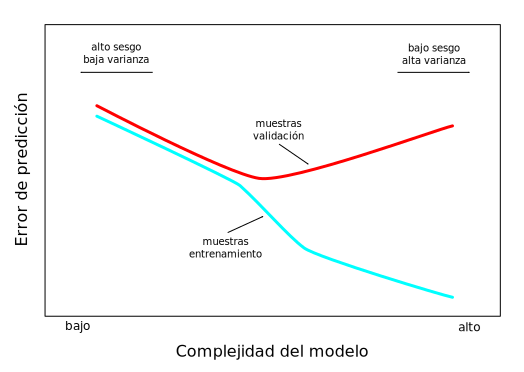
\includegraphics[width=0.9\linewidth]{./figures/complejidad_modelo.pdf}
\caption{Evolución del error en función en las muestras de entrenamiento y validación en función de la complejidad del modelo. The Elements of Statistical Learning, Trevor Hastie.}
\label{fig:complejidad_modelo}
\end{center}
\end{figure}

\subsubsection{\texorpdfstring{Validación cruzada
\emph{leave-one-out}}{Validación cruzada leave-one-out}}\label{validacion-cruzada-leave-one-out}

La validación \emph{leave-one-out} (validación dejando uno fuera) es una
validación muy sencilla pero que computacionalmente puede ser muy
costosa. El procedimiento de la validación \emph{leave-one-out} se basa
en lo siguiente: Si tenemos \emph{n} observaciones entonces construimos
\emph{n} Máquinas de Vector Soporte,
\(\{SVM_1, SVM_2, \ldots, SVM_n\}\), cada una de ellas con \emph{n-1}
muestras, \(SVM_i = \{1, 2, \ldots, i-1, i+1, \ldots, n \}\) y aplicamos
el modelo sobre la muestra no utilizada en la construcción del modelo.

\subsubsection{\texorpdfstring{Validación cruzada
\emph{k-fold}}{Validación cruzada k-fold}}\label{validacion-cruzada-k-fold}

La validación \emph{k-fold} consiste en separar las muestras en \emph{k}
grupos de mismo tamaño. Se construyen entonces \emph{k} Máquinas de
Vector Soporte con \emph{k-1} grupos y se aplica el modelo resultante
sobre el grupo de muestras no incluidas en el modelo. Observamos que si
\emph{k = n} estamos ante la validación \emph{leave-one-out}.

\clearpage
\newpage

\section{\texorpdfstring{Práctica: Construcción de una Máquina de Vector
Soporte con
\texttt{R}}{Práctica: Construcción de una Máquina de Vector Soporte con R}}\label{practica-construccion-de-una-maquina-de-vector-soporte-con-r}

Hay muchos paquetes en \texttt{R} que permiten construir SVM como por
ejemplo el paquete \texttt{e1071} o el paquete \texttt{kernlab}.
Nosotros vamos a trabajar con el paquete \texttt{caret} un paquete
diseñado por \emph{Max Kuhn} precisamente para la búsqueda de modelos,
en particular SVM.

La práctica que vamos a desarrollar consiste en la creación y validación
de una Máquina de Vector Soporte que sea capaz de distinguir el dígito
escrito en una imagen de entre los diez posibles dígitos: 0, 1, 2,
\ldots{}, 8 y 9. Los datos se han generado a partir de 130 imágenes por
cada dígito en las que en cada imagen el dígito está escrito con una
tipografía diferente. El código para generar dichas imágenes está
escrito es el código \ref{cod:extrafont} en el anexo.

En total tenemos 1300 imágenes de 16x16 píxeles cada una, por lo que
tenemos 256 píxeles de información en cada imagen que podemos considerar
como 256 variables. Mediante el programa
\href{http://www.imagemagick.org/}{imageMagick} hemos pasado cada imagen
a información en texto que podemos leer fácilmente con \texttt{R}. En el
código \ref{cod:imagemagick} están descritas las primeras 25 líneas de
uno de los ficheros generados.

\lstinputlisting[language = R, caption = {ImageMagick pixel enumeration: 30, 30, 255, srgb.}, label = cod:imagemagick, linerange = {1-25}]{./code/imagemagick.txt}

El código anterior son las primeras líneas del fichero en texto de una
imagen. La primera fila es la descripción del fichero, la segunda línea
nos informa que el punto (0,0) de la imagen es de color blanco. La
información está en \emph{rgb}, \emph{hexadecimal} y en modo texto
(\emph{white}, \emph{black}). Nosotros utilizaremos la última columna
como la información de nuestras variables.

En la figura \ref{fig:imagenes_8} se muestra como ejemplo las 130
imágenes del dígito 8 que utilizaremos para entrenar y validar el modelo
de Máquinas de Vector Soporte.

\begin{figure}[h]

{\centering \includegraphics[width=0.8\linewidth]{graphics/svm/imagenes_8-1} 

}

\caption{130 gráficos del número ocho con cada fuente.}\label{fig:imagenes_8}
\end{figure}

Dibujamos el perfil promedio de cada dígito. Las figuras, generadas a
16x16 pixeles de resolución nos dan un total de 256 variables en las que
tenemos los valores \emph{white} o \emph{black}, una variable por cada
píxel de la imagen. Nosotros pasaremos estos valores a -1 y 1. Cuanto
mayor sea la resolución de la imagen mayor será también el número de
variables. Las diferencias claras entre los distintos números, que hace
que seamos capaces de distinguirlos, tienen que verse también en el
perfil generado por las 256 variables y estas diferencias son las que
tiene que encontrar la Máquina de Vector Soporte. En la figura
\ref{fig:perfiles_digitos} se muestran la distribución promedio de cada
píxel para cada dígito.

\begin{figure}[h]

{\centering \includegraphics[width=0.8\linewidth]{graphics/svm/perfiles_digitos-1} 

}

\caption{Distribución.}\label{fig:perfiles_digitos}
\end{figure}

\subsection{Support Vector Machine
Learning}\label{support-vector-machine-learning}

Como ya hemos comentado, las máquinas de vector soporte dependen de la
función kernel que consideremos. Las más usuales son las funciones
kernel lineales y las funciones kernel de base radial {[}1{]}. Con los
datos de las 1300 imágenes vamos a construir diferentes Máquinas de
Vector Soporte utilizando diferentes argumentos y parámetros y
compararemos sus resultados.

\subsubsection{Linear Support Vector
Machine}\label{linear-support-vector-machine}

Estimamos la exactitud de una máquina de vector soporte con función
kernel lineal. La forma de atacar este problema por parte de la librería
\texttt{caret} {[}2,3{]} es evaluando cada punto de la malla generada
por los diferentes valores de los parámetros \emph{sigma} (\(\sigma\)) y
\emph{costo} (\(c\)). Una vez evaluados todos los paŕametros elegiremos
aquél par (\emph{sigma}, \emph{costo}) que haya maximizado la exactitud
de las predicciones. Valoramos la construcción del modelo considerando 5
repeticiones con el 80\% del total de la muestra
(\texttt{trainControl(method\ =\ "cv",\ p\ =\ 0.8,\ digito\ =\ 5,\ repeats\ =\ 5,\ search\ =\ "grid")}).
Para evaluar un modelo de máquinas de vector soporte con kernel lineal,
le pasamos a la función \texttt{train} el argumento
\texttt{method\ =\ "svmLinear2"} que será evaluada internamente con las
funciones del paquete \texttt{kernlab} {[}4{]}.

En metabolómica, es habitual realizar diferentes transformaciones en los
datos para conseguir distribuciones normales o distribuciones
tipificadas entre otras muchas {[}5{]}. La función \texttt{train}
permite considerar diferentes transformaciones sobre los datos. Las más
comunes son:

\begin{itemize}
\item
  \textbf{Datos originales}. Trabajaremos con los datos originales, sin
  ningún tipo de preprocesado previo utilizando el comando
  \texttt{preProcess\ =\ NULL}.
\item
  \textbf{Datos escalados y centrados}. Si las variables tienen
  diferentes escalas y variabilidad es interesante considerar el
  centrado de variables y su escalado, para que no influya en el
  análisis. Utilizaremos el comando
  \texttt{preProcess\ =\ c("scale",\ "center")}.
\end{itemize}

\begin{equation}
  X^{\prime} = \dfrac{X -\bar{X}}{\sigma_{X}}
  \end{equation}

\begin{itemize}
\tightlist
\item
  \textbf{Datos transformados según potencias \emph{Box-Cox}}. Las
  transformacion es \emph{Box-Cox} son una familia de transformaciones
  cuya finalidad principal es normalizar una variable. El comando que
  podemos utilizar es \texttt{preProcess\ =\ "BoxCox"}.
\end{itemize}

\begin{equation}
  y_{i}^{(\lambda )}={\begin{cases}{\dfrac {y_{i}^{\lambda }-1}{\lambda }}&{\text{si }}\lambda \neq 0,\\[8pt]\ln {(y_{i})}&{\text{si }}\lambda =0,\end{cases}}
  \end{equation}

\begin{figure}[h]

{\centering \includegraphics[width=0.8\linewidth]{graphics/svm/imagen_digitos_jitter-1} 

}

\caption{Ejemplo  de los dígitos a reconocer tras haber añadido ruido a la imagen.}\label{fig:imagen_digitos_jitter}
\end{figure}

La figura \ref{fig:pca_entrenamiento} muestra la proyección sobre las
dos primeras componentes las observaciones que utilizaremos para
entrenar al modelo (65 observaciones de cada dígito). Vemos que hay una
separación evidente entre algunos dígitos y otros están juntos.
Comprobamos que las observaciones de los dígitos 1 y 7 están cercanas,
así como las observaciones de los dígitos 0, 6 y 8.

Estas diferencias visibles en el Análisis de Componentes Principales ya
nos hacen intuir que un modelo SVM puede tener un gran capacidad de
pronóstico. El código en \texttt{R} para generar el PCA puede
consultarse en el código \ref{cod:pca} en el anexo.

\begin{figure}[h]

{\centering \includegraphics[width=0.95\linewidth]{graphics/svm/pca_entrenamiento-1} 

}

\caption{Análisis de Componentes Principales con 100 observaciones por cada dígito. Comprobamos que las observaciones de los dígitos 1 y 7 están cercanas, así las observaciones de los dígitos 0, 6 y 8. Además, estos dos grupos de observaciones están situados en grupos opuestos en la primera componente, así que podríamos interpretar que la primera componente está relacionada con el volumen del número.}\label{fig:pca_entrenamiento}
\end{figure}

Vamos a aplicar la función \texttt{train()} con el mínimo número de
argumentos:

\begin{itemize}
\item
  \textbf{x}: Matriz de datos.
\item
  \textbf{y}: Clasificación de las muestras.
\item
  \textbf{method}: Una cadena de texto en la que se especifica el modelo
  de clasificación o regresión a considerar. En nuestro caso vamos a
  utilizar \texttt{svmLinear2} que es un \emph{kernel} disponible desde
  la librería \texttt{e1071}.
\end{itemize}

\begin{Shaded}
\begin{Highlighting}[]
\NormalTok{X <-}\StringTok{ }\NormalTok{entrenamiento[, }\DecValTok{1}\OperatorTok{:}\DecValTok{256}\NormalTok{]}
\NormalTok{Y <-}\StringTok{ }\NormalTok{entrenamiento}\OperatorTok{$}\NormalTok{digito}
\NormalTok{modelo <-}\StringTok{ }\KeywordTok{train}\NormalTok{(}\DataTypeTok{x =}\NormalTok{ X,}
                \DataTypeTok{y =}\NormalTok{ Y,}
                \DataTypeTok{method =} \StringTok{"svmLinear2"}\NormalTok{)}
\end{Highlighting}
\end{Shaded}

La función \texttt{train()} devuelve un objeto de la clase
\texttt{train} que es una lista que contiene los siguientes elementos:

\begin{itemize}
\item
  \textbf{method}: El modelo elegido. Es el que hemos pasado como
  argumento.
\item
  \textbf{modelType}: Un identificador del tipo de modelo.
\item
  \textbf{results}: Un \texttt{data.frame} de datos la tasa de error de
  entrenamiento y los valores de los parámetros de ajuste.
\item
  \textbf{bestTune}: Un \texttt{data.frame} de datos con los parámetros
  finales.
\item
  \textbf{metric}: Una cadena de texto que especifica qué métrica de
  resumen se utilizará para seleccionar el modelo óptimo.
\item
  \textbf{control}: La lista de parámetros de control.
\item
  \textbf{preProcess}: \texttt{NULL} o un objeto de clase
  \texttt{preProcess}.
\item
  \textbf{finalModel}: Un objeto de ajuste utilizando los mejores
  parámetros.
\item
  \textbf{trainingData}: Un \texttt{data.frame}.
\item
  \textbf{resample}: Un \texttt{data.frame} con columnas para cada
  métrica de rendimiento. Cada fila corresponde a cada re-muestreo. Si
  se solicitan los métodos de validación cruzada o de validación fuera
  de bolsa, estos valores serán \texttt{NULL}.
\item
  \textbf{perfNames}: Un vector de caracteres de métricas de rendimiento
  que se producen mediante la función \texttt{summary()}.
\item
  \textbf{maximize}: Un valor lógico que proviene de los argumentos de
  la función.
\item
  \textbf{yLimits}: El rango de los resultados del conjunto de
  entrenamiento.
\end{itemize}

Primero, entrenamos una SVM con un \emph{kernel} lineal. En este caso
utilizamos la función \texttt{svmLinear2} del paquete \texttt{e1071}. En
\href{http://topepo.github.io/caret/available-models.html}{modelos
disponibles} se pueden consultar los modelos disponibles. También se
puede ejecutar el comando \texttt{names(getModelInfo())}. Los modelos
específicos para construir Máquinas de Vector Soporte pueden consultarse
en
\href{http://topepo.github.io/caret/train-models-by-tag.html\#support-vector-machines}{train
models}.

En la tabla \ref{tab:train_models} se muestran 16 descritos los métodos
para trabajar con la función \texttt{train()} para construir Máquinas de
Vector Soporte.

\begin{table}[ht]
\centering
\scalebox{0.7}{
\begin{tabular}{p{5cm}p{5cm}p{3cm}p{2cm}p{3cm}}
  \hline
\hline
Model & Method & Type & Libraries & Tuning parameters \\ 
  \hline
L2 Regularized Linear Support Vector Machines with Class Weights & svmLinearWeights2 & Classification & LiblineaR & cost, Loss, weight \\ 
  L2 Regularized Support Vector Machine (dual) with Linear Kernel & svmLinear3 & Classification, Regression & LiblineaR & cost, Loss \\ 
  Least Squares Support Vector Machine & lssvmLinear & Classification & kernlab & tau \\ 
  Least Squares Support Vector Machine with Polynomial Kernel & lssvmPoly & Classification & kernlab & degree, scale, tau \\ 
  Least Squares Support Vector Machine with Radial Basis Function Kernel & lssvmRadial & Classification & kernlab & sigma, tau \\ 
  Linear Support Vector Machines with Class Weights & svmLinearWeights & Classification & e1071 & cost, weight \\ 
  Support Vector Machines with Boundrange String Kernel & svmBoundrangeString & Classification, Regression & kernlab & length, C \\ 
  Support Vector Machines with Class Weights & svmRadialWeights & Classification & kernlab & sigma, C, Weight \\ 
  Support Vector Machines with Exponential String Kernel & svmExpoString & Classification, Regression & kernlab & lambda, C \\ 
  Support Vector Machines with Linear Kernel & svmLinear & Classification, Regression & kernlab & C \\ 
  Support Vector Machines with Linear Kernel & svmLinear2 & Classification, Regression & e1071 & cost \\ 
  Support Vector Machines with Polynomial Kernel & svmPoly & Classification, Regression & kernlab & degree, scale, C \\ 
  Support Vector Machines with Radial Basis Function Kernel & svmRadial & Classification, Regression & kernlab & sigma, C \\ 
  Support Vector Machines with Radial Basis Function Kernel & svmRadialCost & Classification, Regression & kernlab & C \\ 
  Support Vector Machines with Radial Basis Function Kernel & svmRadialSigma & Classification, Regression & kernlab & sigma, C \\ 
  Support Vector Machines with Spectrum String Kernel & svmSpectrumString & Classification, Regression & kernlab & length, C \\ 
   \hline
\hline
\end{tabular}
}
\caption{Modelos disponibles para construir Máquinas de Vector Soporte con la función {\it train()}.} 
\label{tab:train_models}
\end{table}

Tras aplicar la función \texttt{train()} sobre nuestros datos obtenos el
objeto \texttt{modelo}.

\begin{Shaded}
\begin{Highlighting}[]
\KeywordTok{print}\NormalTok{(modelo)}
\end{Highlighting}
\end{Shaded}

\begin{verbatim}
## Support Vector Machines with Linear Kernel 
## 
## 650 samples
## 256 predictors
##  10 classes: '0', '1', '2', '3', '4', '5', '6', '7', '8', '9' 
## 
## No pre-processing
## Resampling: Bootstrapped (25 reps) 
## Summary of sample sizes: 650, 650, 650, 650, 650, 650, ... 
## Resampling results across tuning parameters:
## 
##   cost  Accuracy   Kappa    
##   0.25  0.9859124  0.9843156
##   0.50  0.9859124  0.9843156
##   1.00  0.9859124  0.9843156
## 
## Accuracy was used to select the optimal model using  the largest value.
## The final value used for the model was cost = 0.25.
\end{verbatim}

El modelo con estructura de SVM guardado en \texttt{modelo} es una lista
con varios argumentos.

\begin{Shaded}
\begin{Highlighting}[]
\NormalTok{modelo}\OperatorTok{$}\NormalTok{method}
\end{Highlighting}
\end{Shaded}

\begin{verbatim}
## [1] "svmLinear2"
\end{verbatim}

\begin{Shaded}
\begin{Highlighting}[]
\NormalTok{modelo}\OperatorTok{$}\NormalTok{modelType}
\end{Highlighting}
\end{Shaded}

\begin{verbatim}
## [1] "Classification"
\end{verbatim}

\begin{Shaded}
\begin{Highlighting}[]
\NormalTok{modelo}\OperatorTok{$}\NormalTok{results}
\end{Highlighting}
\end{Shaded}

\begin{verbatim}
##   cost  Accuracy     Kappa  AccuracySD    KappaSD
## 1 0.25 0.9859124 0.9843156 0.009608961 0.01069152
## 2 0.50 0.9859124 0.9843156 0.009608961 0.01069152
## 3 1.00 0.9859124 0.9843156 0.009608961 0.01069152
\end{verbatim}

\begin{Shaded}
\begin{Highlighting}[]
\NormalTok{modelo}\OperatorTok{$}\NormalTok{bestTune}
\end{Highlighting}
\end{Shaded}

\begin{verbatim}
##   cost
## 1 0.25
\end{verbatim}

\begin{Shaded}
\begin{Highlighting}[]
\NormalTok{modelo}\OperatorTok{$}\NormalTok{call}
\end{Highlighting}
\end{Shaded}

\begin{verbatim}
## train.default(x = X, y = Y, method = "svmLinear2")
\end{verbatim}

\begin{Shaded}
\begin{Highlighting}[]
\NormalTok{modelo}\OperatorTok{$}\NormalTok{metric}
\end{Highlighting}
\end{Shaded}

\begin{verbatim}
## [1] "Accuracy"
\end{verbatim}

\begin{Shaded}
\begin{Highlighting}[]
\KeywordTok{names}\NormalTok{(modelo}\OperatorTok{$}\NormalTok{control)}
\end{Highlighting}
\end{Shaded}

\begin{verbatim}
##  [1] "method"            "number"            "repeats"          
##  [4] "search"            "p"                 "initialWindow"    
##  [7] "horizon"           "fixedWindow"       "skip"             
## [10] "verboseIter"       "returnData"        "returnResamp"     
## [13] "savePredictions"   "classProbs"        "summaryFunction"  
## [16] "selectionFunction" "preProcOptions"    "sampling"         
## [19] "index"             "indexOut"          "indexFinal"       
## [22] "timingSamps"       "predictionBounds"  "seeds"            
## [25] "adaptive"          "trim"              "allowParallel"
\end{verbatim}

\begin{Shaded}
\begin{Highlighting}[]
\NormalTok{modelo}\OperatorTok{$}\NormalTok{preProcess}
\end{Highlighting}
\end{Shaded}

\begin{verbatim}
## NULL
\end{verbatim}

\begin{Shaded}
\begin{Highlighting}[]
\NormalTok{modelo}\OperatorTok{$}\NormalTok{finalModel}
\end{Highlighting}
\end{Shaded}

\begin{verbatim}
## 
## Call:
## svm.default(x = as.matrix(x), y = y, kernel = "linear", cost = param$cost, 
##     probability = classProbs)
## 
## 
## Parameters:
##    SVM-Type:  C-classification 
##  SVM-Kernel:  linear 
##        cost:  0.25 
##       gamma:  0.00390625 
## 
## Number of Support Vectors:  419
\end{verbatim}

En la tabla \ref{tab:entrenamiento_modelo_svm_linear2_paso1} se muestra
la matriz de confusión entre los dígitos observados (columnas) y los
dígitos pronosticados (filas) de los 1000 dígitos de los datos
utilizados en el entrenamiento del modelo.

\begin{table}[ht]
\centering
\scalebox{0.8}{
\begin{tabular}{rrrrrrrrrrr}
  \hline
\hline
 & 0 & 1 & 2 & 3 & 4 & 5 & 6 & 7 & 8 & 9 \\ 
  \hline
0 &  65 &   0 &   0 &   0 &   0 &   0 &   0 &   0 &   0 &   0 \\ 
  1 &   0 &  65 &   0 &   0 &   0 &   0 &   0 &   0 &   0 &   0 \\ 
  2 &   0 &   0 &  65 &   0 &   0 &   0 &   0 &   0 &   0 &   0 \\ 
  3 &   0 &   0 &   0 &  65 &   0 &   0 &   0 &   0 &   0 &   0 \\ 
  4 &   0 &   0 &   0 &   0 &  65 &   0 &   0 &   0 &   0 &   0 \\ 
  5 &   0 &   0 &   0 &   0 &   0 &  65 &   0 &   0 &   0 &   0 \\ 
  6 &   0 &   0 &   0 &   0 &   0 &   0 &  65 &   0 &   0 &   0 \\ 
  7 &   0 &   0 &   0 &   0 &   0 &   0 &   0 &  65 &   0 &   0 \\ 
  8 &   0 &   0 &   0 &   0 &   0 &   0 &   0 &   0 &  65 &   0 \\ 
  9 &   0 &   0 &   0 &   0 &   0 &   0 &   0 &   0 &   0 &  65 \\ 
   \hline
\hline
\end{tabular}
}
\caption{Matriz de confusión entre los dígitos observados y los dígitos pronosticados por el modelo.} 
\label{tab:entrenamiento_modelo_svm_linear2_paso1}
\end{table}

En la tabla \ref{tab:validacion_modelo_svm_linear2_paso1} se muestra la
matriz de confusión entre los dígitos observados (columnas) y los
dígitos pronosticados (filas) de los 300 dígitos de los datos utilizados
en la validación del modelo.

\begin{table}[ht]
\centering
\scalebox{0.8}{
\begin{tabular}{rrrrrrrrrrr}
  \hline
\hline
 & 0 & 1 & 2 & 3 & 4 & 5 & 6 & 7 & 8 & 9 \\ 
  \hline
0 &  60 &   0 &   0 &   0 &   0 &   2 &   2 &   0 &   1 &   1 \\ 
  1 &   0 &  64 &   1 &   0 &   0 &   0 &   0 &   1 &   1 &   0 \\ 
  2 &   0 &   0 &  63 &   0 &   0 &   0 &   0 &   0 &   1 &   0 \\ 
  3 &   0 &   0 &   0 &  64 &   0 &   2 &   0 &   0 &   0 &   0 \\ 
  4 &   2 &   0 &   0 &   0 &  65 &   0 &   1 &   0 &   1 &   1 \\ 
  5 &   0 &   0 &   0 &   0 &   0 &  57 &   0 &   0 &   0 &   0 \\ 
  6 &   2 &   0 &   0 &   0 &   0 &   4 &  62 &   0 &   0 &   0 \\ 
  7 &   0 &   1 &   0 &   0 &   0 &   0 &   0 &  64 &   0 &   0 \\ 
  8 &   1 &   0 &   0 &   1 &   0 &   0 &   0 &   0 &  61 &   0 \\ 
  9 &   0 &   0 &   1 &   0 &   0 &   0 &   0 &   0 &   0 &  63 \\ 
   \hline
\hline
\end{tabular}
}
\caption{Matriz de confusión entre los dígitos de validación y los dígitos pronosticados por el modelo.} 
\label{tab:validacion_modelo_svm_linear2_paso1}
\end{table}

Observamos que hay una tasa de error en la validación del 0.09.

\begin{figure}[h]

{\centering \includegraphics[width=0.8\linewidth]{graphics/svm/digitos_fallados_modelo_svm_linear2_paso1_a-1} 

}

\caption{Casos en los que ha fallado el modelo a la hora de interpretar un dígito. El dígito del centro (negrita) representa el número que la Máquina de Vector Soporte no ha sabido interpretar. El dígito de la esquina inferior (gris) representa el dígito que ha predicho el modelo.}\label{fig:digitos_fallados_modelo_svm_linear2_paso1_a}
\end{figure}

\begin{figure}[h]

{\centering \includegraphics[width=0.8\linewidth]{graphics/svm/digitos_fallados_modelo_svm_linear2_paso1_b-1} 

}

\caption{Casos en los que ha fallado el modelo a la hora de interpretar un dígito. Los dígitos se representan tal y como se ven en las imágenes.}\label{fig:digitos_fallados_modelo_svm_linear2_paso1_b}
\end{figure}

Utilizamos la función \texttt{varImp()} del paquete \texttt{caret}. Esta
función tiene como argumento la salida de la función \texttt{train}, es
decir, el modelo construido. La salida de la función \texttt{varImp()}
depende del modelo que sele haya pasado como argumento. En nuestro caso
la salida es una lista de tres elementos:

\begin{itemize}
\item
  \textbf{importance}: Es un \texttt{data.frame} con tantas filas como
  variables y tantas columnas como clases a separar que contiene un
  índice de importancia para discriminar entre clases que va de 0 a 100
  (\texttt{scaled\ =\ TRUE}) .
\item
  \textbf{model}: Modelo que permite calcular el índice de importancia
  entre clases. Por defecto se utiliza un análisis ROC.
\item
  \textbf{calledFrom}: Nos informa de la llamada a la función.
\end{itemize}

En la figura \ref{fig:varimp_modelo_1_modelo_svmlinear2_paso1} se
muestra el gráfico por defecto al dibujar el objeto devuelto por la
función \texttt{varImp()}.

\begin{Shaded}
\begin{Highlighting}[]
\NormalTok{a <-}\StringTok{ }\KeywordTok{varImp}\NormalTok{(modelo)}
\KeywordTok{colnames}\NormalTok{(a}\OperatorTok{$}\NormalTok{importance) <-}\StringTok{ }\KeywordTok{paste}\NormalTok{(}\StringTok{"dígito"}\NormalTok{, }
                                \KeywordTok{seq}\NormalTok{(}\DecValTok{0}\NormalTok{, }\DecValTok{9}\NormalTok{), }
                                \DataTypeTok{sep =} \StringTok{" "}\NormalTok{)}
\KeywordTok{plot}\NormalTok{(a, }\DataTypeTok{top =} \DecValTok{20}\NormalTok{, }
     \DataTypeTok{xlab =} \StringTok{"Variables (píxeles) más importantes"}\NormalTok{)}
\end{Highlighting}
\end{Shaded}

\begin{figure}[h]

{\centering \includegraphics[width=0.8\linewidth]{graphics/svm/varimp_modelo_1_modelo_svmlinear2_paso1-1} 

}

\caption{Las 20 variables más importantes para la discriminación de dígitos, es decir, qué pixeles son más importantes para clasificar.}\label{fig:varimp_modelo_1_modelo_svmlinear2_paso1}
\end{figure}

En la figura \ref{fig:varimp_modelo_2_modelo_svmlinear2_paso1}
representamos la importancia de cada variable como si fueran los píxeles
de una imagen. Como era evidente, los márgenes de las imágenes no son
importantes para discriminar entre los diferentes dígitos (blanco y
gris) y si son más importantes los píxeles centrales de las imágenes
(negro).

\begin{figure}[h]

{\centering \includegraphics[width=0.8\linewidth]{graphics/svm/varimp_modelo_2_modelo_svmlinear2_paso1-1} 

}

\caption{Los píxeles más importantes a la hora de tomar una decisión. En blanco se señalan los píxeles menos significativos y en negro están marcados los más significativos en promedio para discriminar entre dígitos.}\label{fig:varimp_modelo_2_modelo_svmlinear2_paso1}
\end{figure}

\clearpage
\newpage

\subsubsection{Linear Support Vector Machine. Modificación de argumentos
y
parámetros}\label{linear-support-vector-machine.-modificacion-de-argumentos-y-parametros}

En el ejemplo que hemos realizado no hemos modificado ningún parámetro y
todos los argumentos necesarios han sido los que vienen por defecto. En
el siguiente ejemplo añadimos varios párametros más:

\begin{itemize}
\item
  \textbf{preProcess}: Argumento que indica si existe algún
  preprocesamiento previo de los datos. En este casos escalamos y
  centramos las variables. Dada la naturaleza de los datos este proceso
  no va a mejorar los resultados previos, pero con otro tipo de datos
  puede ser interesante. Por defecto, este valor es \texttt{NULL}.
\item
  \textbf{trControl}: Argumento al que se le puede pasar una lista que
  controla el proceso de búsqueda del modelo. En este caso pasamos los
  siguientes controles:

  \begin{itemize}
  \item
    \textbf{method = cv}: Método de remuestreo. Se pueden elegir entre
    varios métodos, algunos específicos del modelo a buscar: svm, rf,
    knn, \ldots{}
  \item
    \textbf{p = 0.8}: Porcentaje de muestras utilizadas en el
    entrenamiento de la validación cruzada.
  \item
    \textbf{number = 5}: Número de iteraciones o número de subgrupos de
    validación (\emph{k}-fold).
  \item
    \textbf{repeats = 5}: Repetición de \emph{k}-fold de la validación
    cruzada. En este caso tomamos \emph{k} = 5.
  \end{itemize}
\item
  \textbf{tuneLength}: Número de veces que se ejecutará la búsqueda de
  un modelo variando los parámetros propios de la función \emph{kernel}.
  En este caso, se variará el parámetro \emph{cost} del \emph{kernel}
  lineal.
\item
  \textbf{metric}: Argumento que le indica a la función cuál va a ser el
  criterio para elegir los valores óptimos del modelo. En el caso
  lineal, nos mostrará cuál es el costo óptimo para el cuál se alcanzará
  la exactitud máxima. Las métricas disponibles son:

  \begin{itemize}
  \item
    \textbf{RMSE} y \(R^2\) para regresión.
  \item
    \textbf{accuracy} y \textbf{kappa} para clasificación.
  \end{itemize}
\item
  \textbf{maximize}: Valor lógico que indica a la función si debe buscar
  el máximo o el mínimo de la métrica. Por ejemplo, buscaremos minimizar
  el \emph{RMSE} en regresión pero maximizaremos el \emph{Accuracy} en
  clasificación.
\end{itemize}

Se pueden consultar las opciones de
\href{http://topepo.github.io/caret/subsampling-for-class-imbalances.html}{remuestreo}.

El siguiente código en \texttt{R} construye una Máquina de Vector
Soporte realizando un pre-procesado de los datos escalándolos y
centrándolos. Además, utiliza un control de validación cruzada, en el
que se usa el 80\% de las muestras

\begin{Shaded}
\begin{Highlighting}[]
\NormalTok{X <-}\StringTok{ }\NormalTok{entrenamiento[, }\DecValTok{1}\OperatorTok{:}\DecValTok{256}\NormalTok{]}
\NormalTok{Y <-}\StringTok{ }\NormalTok{entrenamiento}\OperatorTok{$}\NormalTok{digito}

\NormalTok{modelo <-}\StringTok{ }\KeywordTok{train}\NormalTok{(}\DataTypeTok{x =}\NormalTok{ X,}
                \DataTypeTok{y =}\NormalTok{ Y,}
                \DataTypeTok{preProcess =} \KeywordTok{c}\NormalTok{(}\StringTok{"scale"}\NormalTok{, }\StringTok{"center"}\NormalTok{),}
                \DataTypeTok{trControl =} \KeywordTok{trainControl}\NormalTok{(}\DataTypeTok{method =} \StringTok{"cv"}\NormalTok{,}
                                         \DataTypeTok{p =} \FloatTok{0.8}\NormalTok{, }
                                         \DataTypeTok{number =} \DecValTok{5}\NormalTok{,}
                                         \DataTypeTok{repeats =} \DecValTok{5}\NormalTok{),}
                \DataTypeTok{method =} \StringTok{"svmLinear2"}\NormalTok{,}
                \DataTypeTok{tuneLength =} \DecValTok{10}\NormalTok{,}
                \DataTypeTok{maximize =} \OtherTok{TRUE}\NormalTok{,}
                \DataTypeTok{metric =} \StringTok{"Accuracy"}\NormalTok{)     }
\end{Highlighting}
\end{Shaded}

Tras aplicar la función \texttt{train()} sobre nuestros datos obtenos el
objeto \texttt{modelo}.

\begin{Shaded}
\begin{Highlighting}[]
\KeywordTok{print}\NormalTok{(modelo)}
\end{Highlighting}
\end{Shaded}

\begin{verbatim}
## Support Vector Machines with Linear Kernel 
## 
## 650 samples
## 256 predictors
##  10 classes: '0', '1', '2', '3', '4', '5', '6', '7', '8', '9' 
## 
## Pre-processing: scaled (256), centered (256) 
## Resampling: Cross-Validated (5 fold) 
## Summary of sample sizes: 520, 520, 520, 520, 520 
## Resampling results across tuning parameters:
## 
##   cost    Accuracy   Kappa    
##     0.25  0.9876923  0.9863248
##     0.50  0.9876923  0.9863248
##     1.00  0.9876923  0.9863248
##     2.00  0.9876923  0.9863248
##     4.00  0.9876923  0.9863248
##     8.00  0.9876923  0.9863248
##    16.00  0.9876923  0.9863248
##    32.00  0.9876923  0.9863248
##    64.00  0.9876923  0.9863248
##   128.00  0.9876923  0.9863248
## 
## Accuracy was used to select the optimal model using  the largest value.
## The final value used for the model was cost = 0.25.
\end{verbatim}

En la tabla \ref{tab:validacion_modelo_svm_linear2_paso2} se muestra la
matriz de confusión entre los dígitos observados (columnas) y los
dígitos pronosticados (filas) de los 300 dígitos de los datos utilizados
en la validación del modelo.

\begin{table}[ht]
\centering
\scalebox{0.8}{
\begin{tabular}{rrrrrrrrrrr}
  \hline
\hline
 & 0 & 1 & 2 & 3 & 4 & 5 & 6 & 7 & 8 & 9 \\ 
  \hline
0 &  60 &   0 &   0 &   0 &   0 &   2 &   2 &   0 &   1 &   1 \\ 
  1 &   0 &  64 &   1 &   0 &   0 &   0 &   0 &   1 &   1 &   0 \\ 
  2 &   0 &   0 &  63 &   0 &   0 &   0 &   0 &   0 &   1 &   0 \\ 
  3 &   0 &   0 &   0 &  64 &   0 &   2 &   0 &   0 &   0 &   0 \\ 
  4 &   2 &   0 &   0 &   0 &  65 &   0 &   1 &   0 &   1 &   1 \\ 
  5 &   0 &   0 &   0 &   0 &   0 &  57 &   0 &   0 &   0 &   0 \\ 
  6 &   2 &   0 &   0 &   0 &   0 &   4 &  62 &   0 &   0 &   0 \\ 
  7 &   0 &   1 &   0 &   0 &   0 &   0 &   0 &  64 &   0 &   0 \\ 
  8 &   1 &   0 &   0 &   1 &   0 &   0 &   0 &   0 &  61 &   0 \\ 
  9 &   0 &   0 &   1 &   0 &   0 &   0 &   0 &   0 &   0 &  63 \\ 
   \hline
\hline
\end{tabular}
}
\caption{Matriz de confusión entre los dígitos de validación y los dígitos pronosticados por el modelo.} 
\label{tab:validacion_modelo_svm_linear2_paso2}
\end{table}

\begin{figure}[h]

{\centering \includegraphics[width=0.8\linewidth]{graphics/svm/digitos_fallados_modelo_svm_linear2_paso2_a-1} 

}

\caption{Casos en los que ha fallado el modelo a la hora de interpretar un dígito. El dígito del centro (negrita) representa el número que la Máquina de Vector Soporte no ha sabido interpretar. El dígito de la esquina inferior (gris) representa el dígito que ha predicho el modelo.}\label{fig:digitos_fallados_modelo_svm_linear2_paso2_a}
\end{figure}

\begin{figure}[h]

{\centering \includegraphics[width=0.8\linewidth]{graphics/svm/digitos_fallados_modelo_svm_linear2_paso2_b-1} 

}

\caption{Casos en los que ha fallado el modelo a la hora de interpretar un dígito. Los dígitos se representan tal y como se ven en las imágenes.}\label{fig:digitos_fallados_modelo_svm_linear2_paso2_b}
\end{figure}

Observamos que hay una tasa de error en la validación del 0.09.

\clearpage

\subsection{Conclusiones}\label{conclusiones}

\subsubsection{Ventajas}\label{ventajas}

\begin{itemize}
\item
  Las Máquinas de Vector Soporte trabajan de forma eficiente con grandes
  cantidades de datos.
\item
  Permiten realizar cribados iniciales de variables evaluando la
  importancia de cada una de ellas en la predicción de clases.
\end{itemize}

\subsubsection{Desventajas}\label{desventajas}

\begin{itemize}
\item
  \emph{A priori} no existe un \emph{kernel} óptimo, dependerá de la
  naturaleza de los datos con los que estemos trabajando y siempre será
  recomendable el uso de varios \emph{kernel} y comparar sus resultados.
\item
  La experiencia nos lleva a pensar que las Máquinas de Vector Soporte
  tienden a sobreajustar los datos y siempre es conveniente realizar una
  validación del modelo.
\item
  Los modelos que se obtienen al aplicar una Máquina de Vector Soporte
  suelen ser muy opacos y de dificil interpretación.
\end{itemize}

\clearpage
\newpage

\section{Versión}\label{version}

\begin{itemize}\raggedright
  \item R version 3.3.2 (2016-10-31), \verb|x86_64-pc-linux-gnu|
  \item Locale: \verb|LC_CTYPE=es_ES.UTF-8|, \verb|LC_NUMERIC=C|, \verb|LC_TIME=es_ES.UTF-8|, \verb|LC_COLLATE=es_ES.UTF-8|, \verb|LC_MONETARY=es_ES.UTF-8|, \verb|LC_MESSAGES=es_ES.UTF-8|, \verb|LC_PAPER=es_ES.UTF-8|, \verb|LC_NAME=C|, \verb|LC_ADDRESS=C|, \verb|LC_TELEPHONE=C|, \verb|LC_MEASUREMENT=es_ES.UTF-8|, \verb|LC_IDENTIFICATION=C|
  \item Base packages: base, datasets, graphics, grDevices,
    methods, stats, utils
  \item Other packages: ca~0.70, caret~6.0-76, e1071~1.6-8,
    extrafont~0.17, Formula~1.2-2, ggplot2~2.2.1, Hmisc~4.0-3,
    kernlab~0.9-25, knitr~1.17, lattice~0.20-34, pheatmap~1.0.8,
    pROC~1.10.0, randomForest~4.6-12, RColorBrewer~1.1-2,
    survival~2.41-3, tables~0.8, xtable~1.8-2
  \item Loaded via a namespace (and not attached): acepack~1.4.1,
    backports~1.1.0, base64enc~0.1-3, car~2.1-5, checkmate~1.8.3,
    class~7.3-14, cluster~2.0.5, codetools~0.2-15,
    colorspace~1.2-6, compiler~3.3.2, data.table~1.10.4,
    digest~0.6.8, evaluate~0.10.1, extrafontdb~1.0, foreach~1.4.2,
    foreign~0.8-67, grid~3.3.2, gridExtra~2.2.1, gtable~0.2.0,
    htmlTable~1.9, htmltools~0.3.6, htmlwidgets~0.9,
    iterators~1.0.7, latticeExtra~0.6-28, lazyeval~0.2.0,
    lme4~1.1-13, magrittr~1.5, MASS~7.3-44, Matrix~1.2-7.1,
    MatrixModels~0.4-1, mgcv~1.8-16, minqa~1.2.4,
    ModelMetrics~1.1.0, munsell~0.4.2, nlme~3.1-128, nloptr~1.0.4,
    nnet~7.3-12, parallel~3.3.2, pbkrtest~0.4-7, plyr~1.8.4,
    quantreg~5.33, Rcpp~0.12.12, reshape2~1.4.1, rlang~0.1.2,
    rmarkdown~1.6, rpart~4.1-10, rprojroot~1.2, Rttf2pt1~1.3.4,
    scales~0.5.0, SparseM~1.6, splines~3.3.2, stats4~3.3.2,
    stringi~1.1.5, stringr~1.2.0, tibble~1.3.4, tools~3.3.2,
    yaml~2.1.14
\end{itemize}

\section*{Bibliografía}\label{bibliografia}
\addcontentsline{toc}{section}{Bibliografía}

\hypertarget{refs}{}
\hypertarget{ref-JSSv015i09}{}
{[}1{]} Karatzoglou A, Meyer D, Hornik K. Support vector machines in r.
Journal of Statistical Software {[}Internet{]}. 2006;15:1--28. Available
from:
\url{https://www.jstatsoft.org/index.php/jss/article/view/v015i09}.

\hypertarget{ref-JSSv028i05}{}
{[}2{]} Kuhn M. Building predictive models in r using the caret package.
Journal of Statistical Software {[}Internet{]}. 2008;28:1--26. Available
from:
\url{https://www.jstatsoft.org/index.php/jss/article/view/v028i05}.

\hypertarget{ref-caret2015}{}
{[}3{]} Max Kuhn JW, Weston S, Williams A, et al. Caret: Classification
and regression training {[}Internet{]}. 2015. Available from:
\url{http://CRAN.R-project.org/package=caret}.

\hypertarget{ref-kernlab2004}{}
{[}4{]} Karatzoglou A, Smola A, Hornik K, et al. Kernlab -- an S4
package for kernel methods in R. Journal of Statistical Software
{[}Internet{]}. 2004;11:1--20. Available from:
\url{http://www.jstatsoft.org/v11/i09/}.

\hypertarget{ref-vandenBerg2006}{}
{[}5{]} Berg RA van den, Hoefsloot HCJ, Westerhuis JA, et al. Centering,
scaling, and transformations: Improving the biological information
content of metabolomics data. BMC Genomics {[}Internet{]}. 2006;7:142.
Available from: \url{http://dx.doi.org/10.1186/1471-2164-7-142}.

\hypertarget{ref-krzywinskipostd2014}{}
{[}6{]} Krzywinski M, Altman N. Points of significance: Two-factor
designs. Nature Methods. 2014;11:1187--1188.

\hypertarget{ref-altmanslr2015}{}
{[}7{]} Altman N, Krzywinski M. Simple linear regression. Nature
Methods. 2015;12:999--1000.

\hypertarget{ref-altman2016a}{}
{[}8{]} Altman N, Krzywinski M. Points of significance: Analyzing
outliers: Influential or nuisance? Nature Methods. 2016;13:281--282.

\hypertarget{ref-altman2016b}{}
{[}9{]} Altman N, Krzywinski M. Points of significance: Regression
diagnostics. Nature Methods. 2016;13:385--386.

\hypertarget{ref-kuehl2001}{}
{[}10{]} Kuehl R, Osuna M. Diseño de experimentos: Principios
estadísticos de diseño y análisis de investigación. International
Thomson Editores, S. A. de C. V. 2001.

\hypertarget{ref-pulido2004}{}
{[}11{]} Pulido H, Vara Salazar R de la, González P, et al. Análisis y
diseño de experimentos. McGraw-Hill; 2004.

\hypertarget{ref-martinezarranz2015}{}
{[}12{]} Martínez-Arranz I, Mayo R, Pérez-Cormenzana M, et al. Enhancing
metabolomics research through data mining. Journal of Proteomics.
2015;127, Part B:275--288.

\hypertarget{ref-xie2014}{}
{[}13{]} Xie Y. Knitr: A comprehensive tool for reproducible research in
R. In: Stodden V, Leisch F, Peng RD, editors. Implementing reproducible
computational research {[}Internet{]}. Chapman; Hall/CRC; 2014.
Available from:
\url{http://www.crcpress.com/product/isbn/9781466561595}.

\hypertarget{ref-xie2015}{}
{[}14{]} Xie Y. Dynamic documents with R and knitr {[}Internet{]}. 2nd
ed. Boca Raton, Florida: Chapman; Hall/CRC; 2015. Available from:
\url{http://yihui.name/knitr/}.

\hypertarget{ref-xie2016package}{}
{[}15{]} Xie Y. Knitr: A general-purpose package for dynamic report
generation in r {[}Internet{]}. 2016. Available from:
\url{http://yihui.name/knitr/}.

\hypertarget{ref-armitage2014}{}
{[}16{]} Armitage EG, Barbas C. Metabolomics in cancer biomarker
discovery: Current trends and future perspectives. J Pharm Biomed Anal.
2014;87:1--11.

\hypertarget{ref-miroslava2013}{}
{[}17{]} Čuperlović-Culf M. 5 - metabolomics data analysis -- processing
and analysis of a dataset. In: Čuperlović-Culf M, editor. \{NMR\}
metabolomics in cancer research {[}Internet{]}. Woodhead Publishing;
2013. pp. 261--333. Available from:
\url{http://www.sciencedirect.com/science/article/pii/B9781907568848500056}.

\hypertarget{ref-fox1997}{}
{[}18{]} Fox J. Applied regression analysis, linear models, and related
methods. SAGE Publications; 1997.

% 
%

\clearpage

\section{Apéndices}

\lstinputlisting[language = R, caption = {Implementación de la función {\tt ksvm()} en el paquete {\tt kernlab} de {\tt R} para representar las líneas de separación de clasificación.}, label = cod:kernel_lineal]{./code/kernel_lineal.R}

\lstinputlisting[language = R, caption = {Implementación de la función {\tt ksvm()} en el paquete {\tt kernlab} de {\tt R} para representar las líneas de separación de clasificación.}, label = cod:kernel_cuadratico]{./code/kernel_cuadratico.R}

\lstinputlisting[language = R, caption = {Código para realizar un análisis de componentes principales considerando el dígito que representa cada observación.}, label = cod:pca]{./code/pca.R}

\lstinputlisting[language = R, caption = {Código para construir una máquina de vector soporte con kernel lineal.}, label = cod:modelo_svmlinear2_paso1]{./code/modelo_svmlinear2_paso1.R}

\lstinputlisting[language = R, caption = {Código para construir una máquina de vector soporte con kernel lineal utilizando diferentes argumentos de la función train().}, label = cod:modelo_svmlinear2_paso2]{./code/modelo_svmlinear2_paso2.R}

\lstinputlisting[language = R, caption = {Secuencia de comandos para listar todas las fuentes instaladas en el sistema y generar una imagen de cada dígito (0-9) con cada tipografía. La secuencia de comandos utiliza el paquete extrafont que es específico de Linux, en Windows se debe utilizar la función windowFonts() del paquete grDevices.}, label = cod:extrafont, linerange = {1-17}]{./code/extrafont.R}

%La secuencia de comandos de interfaz de usuario (UI - User Interface) controla el diseño y el aspecto de la aplicación. Se define en una secuencia de comandos en origen denominado \texttt{ui.R}. Aquí está la secuencia de comandos para la aplicación desarrolla en \texttt{Shiny}.

%\lstinputlisting[language = R, caption = {La secuencia de comandos de interfaz de usuario (UI - User Interface) controla el diseño y el aspecto de la aplicación. Se define en una secuencia de comandos en origen denominado \texttt{ui.R}. Aquí está la secuencia de comandos para la aplicación desarrolla en \texttt{Shiny}.}, label = cod:ui]{../app/ui.R}

%La secuencia de comandos \texttt{server.R} contiene las instrucciones que el ordenador necesita para ejecutar la aplicación. Esta es la secuencia de comandos para la aplicación desarrollada en \texttt{Shiny}.

%\lstinputlisting[language = R, caption = {La secuencia de comandos \texttt{server.R} contiene las instrucciones que el ordenador necesita para ejecutar la aplicación. Esta es la secuencia de comandos para la aplicación desarrollada en \texttt{Shiny}.}, label = cod:server]{../app/server.R}

%\subsection{Apéndice 2}\label{apendice2}

%Si consideramos \texttt{R} como un lenguaje de programación, vemos que es un lenguaje de Programación Orientado a Objetos (POO) y es útil aprovecharse de estas características para generar código más ágil y eficaz que trabajando, por ejemplo, con listas u otros objetos de \texttt{R}. También podemos utilizar funciones para crear clases de referencia, como por ejemplo \texttt{SetRefClass}. Además de generar una clase, \texttt{R} nos da la posibilidad de programar métodos específicos para esa clase.

%En el código \ref{cod:class} se muestra la creación en \texttt{R} de la clase \texttt{InfObsModLin}, una clase para trabajar modelos lineales con una única variable independiente, así como diferentes métodos aplicables a esta clase. Estos métodos son:

%\begin{itemize}
% \item {\bfseries initialize()}: Se inicia una clase con unos valores por defecto.
% \item {\bfseries new()}: Se crea una clase con los valores pasados como argumento.
% \item {\bfseries finalize()}: Se imprime en pantalla la clase.
% \item {\bfseries summary.influence()}: Se imprime en pantalla o devuelve la matriz de influencia calculada con la función \texttt{influence.measures()} de los valores de la clase.
% \item{\bfseries summary.model()}: Se immprime en pantalla o devuelve un resumen de las características del modelo generado con los datos de la clase. Tiene un argumento, \texttt{loo=FALSE} (por defecto), que nos devuelve el resumen del modelo calculado con todas las observaciones. Si \texttt{loo=TRUE} nos devuelve el resumen de {\itshape n} modelos calculados con {\itshape n-1} observaciones.
% \item {\bfseries plotdata()}: Se realizan seis gráficos con los valores de influencia de cada observación de la clase. 
%\end{itemize}


%\lstinputlisting[language = R, caption = {Código en \texttt{R} para generar las clase \texttt{InfObsModLin} y diferentes métodos para usar con dicha clase.}, label = cod:class, linerange = {1-178}]{./code/class.R}


\end{document}
